\documentclass[12pt, a4paper]{article}
\usepackage[top=3cm, bottom=3cm, left=3cm, right=3cm]{geometry}
\usepackage[T1]{fontenc}
\usepackage[utf8]{inputenc}
\usepackage[bahasa]{babel}
\usepackage{times}
\usepackage{graphicx}
\usepackage{amsmath, amssymb}
\usepackage{booktabs}
\usepackage{longtable}
\usepackage{enumitem}
\usepackage{hyperref}
\usepackage{setspace}
\onehalfspacing

\setlength{\parindent}{1.25cm}
\setlength{\parskip}{0pt}

% --- Remove numbering from sections for proposal style ---
\renewcommand{\thesection}{}
\renewcommand{\thesubsection}{}
\renewcommand{\thesubsubsection}{}

\begin{document}

% ================================================================
%  METODE PENELITIAN
% ================================================================
\section{METODE PENELITIAN}

\subsection{Tempat dan Waktu Penelitian}

Penelitian ini dilaksanakan dalam dua tahap utama yang mencakup kegiatan eksperimental dan komputasional. Tahap eksperimental meliputi preparasi sampel yang dilakukan di \textbf{Laboratorium Material, FMIPA Universitas Syiah Kuala}, serta akuisisi data spektrum LIBS yang dilaksanakan di \textbf{Laboratorium Optika dan Aplikasi Laser, FMIPA Universitas Syiah Kuala}. Laboratorium ini dilengkapi dengan sistem LIBS berbasis laser Nd:YAG dan spektrometer Echelle yang telah digunakan dalam berbagai studi spektroskopi sebelumnya \cite{mitaphonna2023, mitaphonna2024, khumaeni2025}. Pengukuran komposisi unsur sebagai data referensi (\textit{ground-truth}) menggunakan instrumen X-Ray Fluorescence (XRF) dilakukan di fasilitas analisis yang tersedia di lingkungan Universitas Syiah Kuala.

Tahap komputasional---yang mencakup pembangkitan data sintetis, pengembangan arsitektur model CNN--Transformer encoder--decoder, serta seluruh siklus pelatihan dan evaluasi---dilaksanakan menggunakan \textbf{GPU Compute Server} yang tersedia di laboratorium penelitian. Keseluruhan penelitian direncanakan berlangsung selama \textbf{10 bulan}, dari Februari 2025 hingga November 2025, dengan rincian per fase disajikan pada bagian Jadwal Penelitian.


\subsection{Alat dan Bahan Penelitian}

Peralatan dan bahan yang digunakan dalam penelitian ini disajikan pada Tabel~\ref{tab:alat-bahan}.

\begin{table}[htbp]
\centering
\caption{Alat dan Bahan Penelitian}
\label{tab:alat-bahan}
\small
\begin{tabular}{clll}
\toprule
\textbf{No} & \textbf{Alat/Bahan} & \textbf{Spesifikasi} & \textbf{Jumlah} \\
\midrule
1  & Laser Nd:YAG              & Q-switched, $\lambda$ = 1064 nm, 114 mJ   & 1 unit \\
2  & Lensa bikonveks           & $f$ = 155 mm (pemfokusan laser)            & 1 unit \\
3  & Spektrometer Echelle + OMA& Rentang spektral 200--900 nm               & 1 unit \\
4  & Kabel serat optik         & Penghantar sinyal emisi plasma             & 1 unit \\
5  & Mesin \textit{hydraulic press} & Tekanan hingga 7 ton                  & 1 unit \\
6  & Mortar dan pestel         & Penggerusan sampel tanah                   & 1 set  \\
7  & Ayakan 40 mesh            & 420 $\mu$m                                 & 1 unit \\
8  & Cetakan sampel            & Pembuatan pelet ($\sim$4 mm)               & 1 unit \\
9  & Masker pelindung          & Keselamatan kerja                          & Secukupnya \\
10 & GPU Compute Server        & Pelatihan CNN--Transformer                 & 1 unit \\
11 & Instrumen XRF             & \textit{Ground-truth} konsentrasi elemen   & 1 unit \\
12 & Sampel tanah vulkanik     & G. Seulawah Agam (4 arah $\times$ 3 kedalaman) & \textbf{24 sampel} \\
\bottomrule
\end{tabular}
\end{table}


\subsection{Prosedur Penelitian}

Prosedur pelaksanaan penelitian ini terdiri dari beberapa tahapan utama sebagaimana diilustrasikan dalam diagram alir pada Gambar~\ref{fig:diagram-alir}. Penelitian mengikuti alur kerja yang mengintegrasikan pendekatan berbasis simulasi fisika plasma dengan teknik \textit{deep learning}, di mana keterbatasan jumlah data eksperimental (24 sampel) diatasi dengan memanfaatkan pengetahuan fisika plasma melalui data sintetis \cite{wang2024, favre2025b} sebelum mentransfer representasi yang telah dipelajari ke domain eksperimental.

\begin{figure}[htbp]
    \centering
    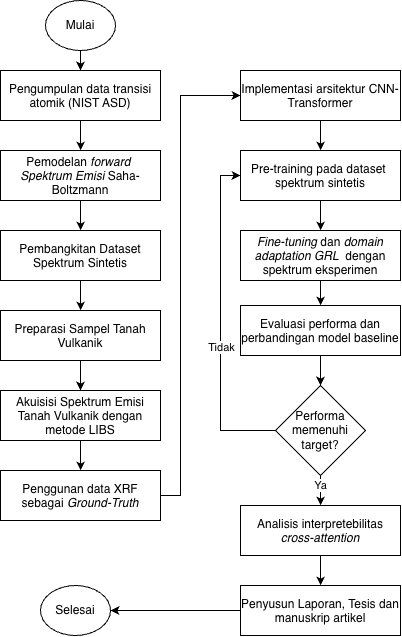
\includegraphics[width=0.55\textwidth]{diagram-alir-M.png}
    \caption{Diagram alir penelitian.}
    \label{fig:diagram-alir}
\end{figure}

% ----------------------------------------------------------------
\subsubsection{Pembangkitan Data Sintetis}

Keterbatasan utama dalam pengembangan model \textit{deep learning} untuk analisis LIBS adalah minimnya ketersediaan data eksperimental berlabel yang memadai untuk pelatihan. Untuk mengatasi hal ini, penelitian ini memanfaatkan \textit{forward model} berbasis fisika plasma untuk membangkitkan dataset sintetis berskala besar. Pendekatan ini telah terbukti efektif dalam meningkatkan kemampuan generalisasi model melalui \textit{pre-training} pada data sintetis sebelum \textit{fine-tuning} pada data eksperimental \cite{wang2024, favre2025b}. Tahapan pembangkitan data sintetis adalah sebagai berikut:

\begin{enumerate}[label=\arabic*., leftmargin=2cm]
    \item \textbf{Pengumpulan data transisi atomik} dari NIST Atomic Spectra Database \cite{kramida2024}: panjang gelombang transisi ($\lambda_{ki}$), koefisien Einstein ($A_{ki}$), degenerasi ($g_i$), dan energi level ($E_i$). Agar rentang simulasi bersifat representatif, parameter elemen dikompilasi secara spesifik untuk \textbf{8 elemen mayor} dan \textbf{15 elemen jejak (\textit{trace elements})} khas tanah vulkanik, dengan batasan rentang konsentrasi sesuai Tabel~\ref{tab:komposisi-tanah}.

\begin{table}[htbp]
\centering
\caption{Rentang referensi komposisi elemen untuk tanah vulkanik yang digunakan dalam pembangkitan dataset spektral sintetis. Elemen dikelompokkan menjadi elemen mayor dan elemen jejak berdasarkan profil geokimia khas tanah vulkanik dan observasi eksperimental XRF.}
\label{tab:komposisi-tanah}
\small
\begin{tabular}{lllp{6cm}}
\toprule
\textbf{Grup} & \textbf{Elemen} & \textbf{Rentang Komposisi (\%)} & \textbf{Peran / Catatan} \\
\midrule
\multicolumn{4}{l}{\textbf{Elemen Mayor (\textit{Major Elements} --- Komponen matriks utama)}} \\
Mayor & Si & 40 -- 60 & Komponen silikat dominan \\
Mayor & Al & 10 -- 18 & Mineral aluminosilikat / feldspar \\
Mayor & Fe & 5 -- 15 & Oksida besi dan mineral feromagnesia \\
Mayor & Ca & 3 -- 10 & Plagioklas dan mineral karbonat \\
Mayor & Mg & 2 -- 8 & Mineral olivin dan piroksen \\
Mayor & Na & 1 -- 5 & Komponen feldspar alkali \\
Mayor & K & 1 -- 5 & Feldspar kalium \\
Mayor & Ti & 0.5 -- 2 & Mineral oksida (ilmenit / rutil) \\
\midrule
\multicolumn{4}{l}{\textbf{Elemen Jejak (\textit{Trace Elements} --- Elemen minor dan penyerta)}} \\
Jejak & Mn & 0.05 -- 0.5 & Berasosiasi dengan mineral Fe \\
Jejak & P & 0.05 -- 0.5 & Mineral apatit \\
Jejak & Ba & 0.01 -- 0.3 & Elemen jejak asosiasi alkali \\
Jejak & Sr & 0.01 -- 0.2 & Mensubstitusi Ca dalam feldspar \\
Jejak & Zn & 0.005 -- 0.1 & Elemen jejak sulfida / oksida \\
Jejak & Cu & 0.001 -- 0.05 & Logam jejak sulfida \\
Jejak & Ni & 0.001 -- 0.05 & Asosiasi mineral mafik \\
Jejak & Cr & 0.001 -- 0.05 & Indikator mineral ultramafik \\
Jejak & V & 0.001 -- 0.05 & Logam transisi pada mineral mafik \\
Jejak & Rb & 0.001 -- 0.05 & Elemen alkali dalam feldspar \\
Jejak & Pb & 0.001 -- 0.02 & Logam jejak berat \\
Jejak & Co & 0.001 -- 0.02 & Berasosiasi dengan mineral Fe \\
Jejak & Mo & 0.0005 -- 0.01 & Logam jejak minor \\
Jejak & Y & 0.0005 -- 0.01 & Berasosiasi dengan \textit{rare earth element} (REE) \\
Jejak & Zr & 0.001 -- 0.02 & Mineral penyerta zirkon \\
\bottomrule
\end{tabular}
\end{table}

    \item \textbf{Penghitungan populasi} tiap tingkat ionisasi menggunakan Persamaan Saha dan distribusi keadaan tereksitasi menggunakan Distribusi Boltzmann \cite{fujimoto2004}. Parameter plasma di-sampling secara acak seragam: $T_e \in [6.000\text{--}15.000]$ K, $n_e \in [10^{16}\text{--}10^{17}]$ cm$^{-3}$. Rentang ini dipilih berdasarkan kondisi tipikal plasma LIBS pada tekanan atmosfer \cite{cristoforetti2010}, dengan mempertimbangkan variasi yang mungkin terjadi pada berbagai jenis matriks sampel.

    \item \textbf{Pembangkitan spektrum monoatomik} $S_\mathrm{mono}^{(z)}(\lambda)$ per elemen dengan menjumlahkan koefisien emisi spektral menggunakan profil Voigt---konvolusi pelebaran Doppler dan Stark broadening \cite{griem1974}. Profil Voigt dipilih karena merepresentasikan mekanisme pelebaran garis spektral dominan pada plasma LIBS, yaitu pelebaran termal (Doppler) dan pelebaran akibat interaksi elektron (Stark).

    \item \textbf{Konstruksi spektrum poliatomik}:
    \begin{equation}
        S_\mathrm{poly}(\lambda) = \sum_{z} c_z \cdot S_\mathrm{mono}^{(z)}(\lambda)
    \end{equation}
    yaitu superposisi terbobot konsentrasi fraksional. Tahap ini secara eksplisit mengimplementasikan hipotesis dekomposisi mono--poliatomik yang menjadi dasar arsitektur encoder--decoder.

    \item \textbf{Konvolusi instrumental} dengan fungsi Gaussian (FWHM = 0{,}02 nm) untuk mencocokkan resolusi spektrometer Echelle yang digunakan dalam eksperimen.

    \item Total dataset yang dibangkitkan: \textbf{10.000 pasangan spektrum sintetis} (monoatomik + poliatomik beserta label konsentrasi dan parameter plasma), dibagi menjadi 80\% untuk \textit{training} dan 20\% untuk \textit{test}.
\end{enumerate}


% ----------------------------------------------------------------
\subsubsection{Akuisisi Data Eksperimental dan Pemodelan}

\paragraph{2a. Sampel Penelitian.}
Penelitian ini memanfaatkan \textbf{24 sampel tanah vulkanik} yang telah dikumpulkan dan dipreparasi dalam rangka program riset kolaboratif grup Laboratorium Optika dan Aplikasi Laser, FMIPA USK. Sampel berasal dari lereng \textbf{Gunung Seulawah Agam, Kabupaten Aceh Besar, Provinsi Aceh}, yang diambil pada \textbf{4 arah mata angin} (Utara, Barat, Selatan, Timur) dan \textbf{3 kedalaman} (0--20 cm, 20--40 cm, 40--60 cm) di setiap titik, sehingga merepresentasikan variasi spasial komposisi geokimia secara sistematis. Strategi pengambilan sampel ini konsisten dengan pendekatan yang digunakan oleh Khumaeni et al. \cite{khumaeni2025} pada studi tanah vulkanik Merapi.

Sampel telah dipreparasi menjadi bentuk pelet pada studi sebelumnya melalui prosedur standar:
\begin{itemize}[leftmargin=2cm]
    \item Pengeringan pada suhu ruang untuk menghilangkan kelembaban berlebih.
    \item Penggerusan hingga halus menggunakan mortar dan pestel.
    \item Penyaringan menggunakan ayakan 40 mesh (420 $\mu$m) untuk menyeragamkan ukuran partikel.
    \item Penimbangan sebanyak kurang lebih 3 gram bubuk per sampel.
    \item Pengepresan menggunakan mesin \textit{hydraulic press} dengan tekanan 7 ton selama 5 menit hingga terbentuk pelet dengan ketebalan sekitar 4 mm.
\end{itemize}

Ketersediaan sampel pelet yang telah terpreparasi memungkinkan penelitian ini untuk langsung berfokus pada tahap akuisisi spektrum LIBS baru dan pengembangan model \textit{deep learning}.


\paragraph{2b. Akuisisi Data Spektrum LIBS Baru.}
Meskipun estimasi komposisi (Tabel~\ref{tab:komposisi-tanah}) dan data baseline awal bersumber dari observasi XRF dan CF-LIBS studi terdahulu, standar kualitas data spektral eksperimental masa lalu belum optimal untuk skenario pelatihan komputasi modern. Oleh karena itu, akuisisi spektrum LIBS \textbf{dilakukan secara baru dan independen} terhadap 24 sampel pelet tersebut. Fokus pembaruan eksperimen terletak pada peningkatan agregasi pengukuran: \textbf{jumlah tembakan laser (\textit{shots})} akan diperbanyak secara masif. Penambahan akumulasi tembakan ini sangat esensial untuk mengatasi fluktuasi ketidakstabilan plasma dan menekan profil \textit{noise} temporal. Hasilnya, \textit{Signal-to-Noise Ratio} (SNR) akan meningkat drastis, sehingga jaringan \textit{deep learning} kelak dapat mendeteksi intensitas emisi lemah secara akurat tanpa tertukar dengan \textit{noise}.

Pengukuran dilaksanakan menggunakan sistem LIBS di Laboratorium Optika dan Aplikasi Laser, FMIPA USK. Prosedur pengambilan datanya adalah sebagai berikut:
\begin{itemize}[leftmargin=2cm]
    \item Berkas laser Nd:YAG ($\lambda$ = 1064 nm, energi pulsa 114 mJ) difokuskan pada permukaan sampel pelet menggunakan lensa bikonveks ($f$ = 155 mm) untuk membangkitkan plasma.
    \item Serat optik dihubungkan ke sistem spektrograf dan diarahkan ke bilik sampel untuk menangkap emisi plasma.
    \item Sampel pelet diposisikan di dalam bilik sampel dan jarak fokus disesuaikan untuk memperoleh intensitas plasma yang ideal.
    \item Emisi plasma tertangkap akan direkam menggunakan \textit{Optical Multichannel Analyzer} (OMA) berbasis spektrometer Echelle (rentang 200--900 nm).
    \item Setiap sampel diablasi dengan \textbf{kuantitas tembakan (\textit{multiple shots}) tinggi} pada \textit{crater} / permukaan titik yang berbeda, lalu semua tangkapan spektral dirata-ratakan secara presisi guna memperoleh stabilitas \textit{continuum} \textit{background} dan ketajaman puncak.
    \item Data spektrum yang terekam ditampilkan dan disimpan menggunakan komputer untuk analisis lebih lanjut.
    \item Garis-garis emisi diidentifikasi menggunakan database NIST Atomic Spectra Database \cite{kramida2024}.
\end{itemize}


\paragraph{2c. Data Ground-Truth Konsentrasi (XRF).}
Data konsentrasi elemen untuk seluruh 24 sampel telah tersedia dari pengukuran \textbf{X-Ray Fluorescence (XRF)} yang dilakukan pada studi sebelumnya dalam program riset grup. Data XRF ini digunakan dalam penelitian ini sebagai \textit{ground-truth} konsentrasi unsur untuk supervisi pada tahap \textit{fine-tuning} model. Penggunaan data XRF yang sudah ada memastikan konsistensi referensi antara studi terdahulu dan penelitian ini, serta menghindari pengulangan pengukuran yang tidak diperlukan. XRF dipilih sebagai referensi karena kemampuannya memberikan analisis kuantitatif multi-elemen yang akurat secara non-destruktif.


\paragraph{2d. Arsitektur Model CNN--Transformer Encoder--Decoder.}
Arsitektur model yang diusulkan dalam penelitian ini dirancang berdasarkan prinsip dekomposisi spektral mono--poliatomik eksplisit, di mana spektrum campuran poliatomik dimodelkan sebagai superposisi terbobot dari spektrum monoatomik penyusunnya. Secara teknis, rancangan jaringan ini ditunjukkan secara menyeluruh pada Gambar~\ref{fig:arsitektur-cnn-trans}. Arsitektur encoder--decoder dipilih karena secara natural mampu memodelkan hubungan antara komponen individu (monoatomik via encoder) dan campurannya (poliatomik via decoder) melalui mekanisme \textit{cross-attention} \cite{vaswani2017, liu2026}. 

\begin{figure}[htbp]
    \centering
    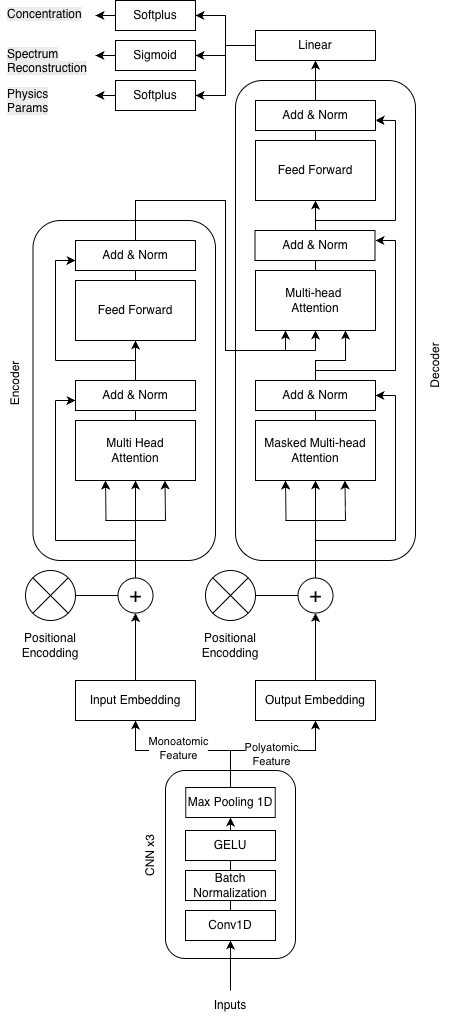
\includegraphics[height=12cm]{Arsitektur-CNN-Trans.png}
    \caption{Representasi visual Arsitektur CNN--Transformer Encoder--Decoder untuk analisis spektral LIBS. Blok ekstrasi fitur 1D CNN dimanfaatkan untuk mereduksi sekuens panjang gelombang sebelum memasuki lapisan atensi Transformer.}
    \label{fig:arsitektur-cnn-trans}
\end{figure}

Komponen utamanya adalah sebagai berikut:

\begin{enumerate}[label=\arabic*., leftmargin=2cm]
    \item \textbf{1D-CNN Feature Extractor} (\textit{shared} encoder--decoder): Dieksekusi secara berulang sebanyak 3 kali blok tumpukan (terdiri dari Conv1D $\rightarrow$ Batch Normalization $\rightarrow$ GELU $\rightarrow$ Max Pooling 1D). Blok ini secara krusial menangkap fitur lokal profil emisi/bentuk garis dan mereduksi resolusi spasial sekuens panjang gelombang.

    \item \textbf{Transformer Encoder} (4 layer, 8 attention heads): menerima fitur CNN dari \textbf{seluruh} spektrum monoatomik (\textit{concatenated}) + \textit{positional} \& \textit{element-type embedding} $\rightarrow$ menghasilkan representasi laten spesifik-elemen via \textit{self-attention}. Encoder mempelajari bagaimana setiap elemen berkontribusi terhadap sinyal spektral secara individual.

    \item \textbf{Transformer Decoder} (4 layer, 8 heads): menerima fitur CNN spektrum campuran poliatomik $\rightarrow$ \textbf{\textit{masked self-attention}} $\rightarrow$ \textbf{\textit{cross-attention}} terhadap output encoder $\rightarrow$ mempelajari aturan komposisi spektral. Mekanisme \textit{cross-attention} memungkinkan decoder untuk meng-query representasi elemen dari encoder dan menentukan kontribusi masing-masing elemen terhadap spektrum campuran yang diamati.

    \item \textbf{Regression Head}: Global Average Pooling $\rightarrow$ Linear projection $\rightarrow$ vektor konsentrasi $\hat{\mathbf{c}} \in \mathbb{R}^Z$.

    \item \textbf{Tiga output head}: (i) konsentrasi elemen (aktivasi Softplus), (ii) rekonstruksi spektrum (Sigmoid), (iii) parameter plasma $T_e$, $n_e$ (Softplus). Desain \textit{multi-task} ini mendorong model untuk tidak hanya memprediksi konsentrasi, tetapi juga mempertahankan konsistensi dengan fisika plasma yang mendasarinya.
\end{enumerate}


\paragraph{2e. Strategi Pelatihan.}
Strategi pelatihan model dirancang dalam tiga fase berurutan untuk memaksimalkan transfer pengetahuan dari domain sintetis ke domain eksperimental. Skema komplit dari alur adaptasi domain ini dapat dilihat pada Gambar~\ref{fig:domain-adapt}.

\begin{figure}[htbp]
    \centering
    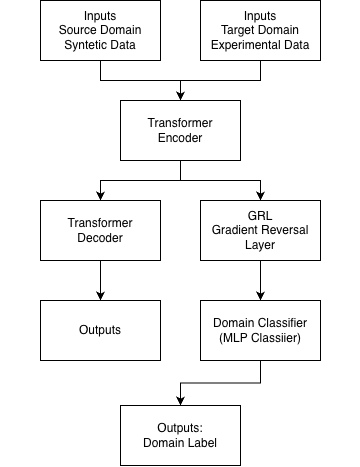
\includegraphics[height=8.5cm]{Domain-Adapt.png}
    \caption{Skema \textit{Domain Adaptation} menggunakan \textit{Gradient Reversal Layer} (GRL). Arsitektur ini memaksa \textit{Transformer Encoder} untuk menghasilkan representasi fitur laten yang tidak bisa dibedakan oleh \textit{Domain Classifier}, sehingga menjembatani \textit{domain gap} antara spektrum sintetis dan eksperimental.}
    \label{fig:domain-adapt}
\end{figure}

\begin{enumerate}[label=\arabic*., leftmargin=2cm]
    \item \textbf{Pre-training} pada data sintetis: 200 epoch, learning rate $10^{-4}$, optimizer Adam \cite{kingma2015} dengan \textit{cosine annealing schedule} \cite{loshchilov2017}. Fungsi loss gabungan digunakan:
    \begin{equation}
        \mathcal{L} = \mathrm{MSE}_\mathrm{konsentrasi} + \alpha \times \mathrm{MSE}_\mathrm{rekonstruksi\;spektral} \quad (\alpha = 0{,}1)
    \end{equation}
    Komponen rekonstruksi spektral berfungsi sebagai regularisasi fisika, memastikan model memetakan fitur spektral yang bermakna secara fisik.

    \item \textbf{Fine-tuning} pada data eksperimental LIBS: 50 epoch, learning rate $10^{-5}$ (lebih rendah untuk mencegah \textit{catastrophic forgetting}), dengan target \textit{ground-truth} konsentrasi dari pengukuran XRF.

    \item \textbf{Domain adaptation}: Gradient Reversal Layer (GRL) \cite{ganin2016} + domain classifier (sintetis vs eksperimental) diintegrasikan selama pelatihan untuk mendorong encoder menghasilkan representasi yang \textit{domain-invariant}. Pendekatan ini mengatasi \textit{domain gap} antara spektrum sintetis (yang mengasumsikan LTE ideal) dan spektrum eksperimental (yang mengandung noise, fluktuasi tembakan-ke-tembakan, dan deviasi dari LTE).
\end{enumerate}


\paragraph{2f. Pengolahan dan Analisis Data.}
Hasil eksperimen dianalisis melalui beberapa tahap:
\begin{itemize}[leftmargin=2cm]
    \item \textbf{Pra-pemrosesan spektrum}: normalisasi intensitas, koreksi \textit{baseline}, dan segmentasi rentang panjang gelombang yang relevan.
    \item \textbf{Identifikasi garis emisi}: pencocokan puncak emisi dengan database NIST ASD untuk verifikasi keberadaan elemen target.
    \item \textbf{Inferensi model}: spektrum eksperimental yang telah di-pra-proses dimasukkan ke model CNN--Transformer yang telah dilatih untuk memprediksi konsentrasi elemen.
    \item \textbf{Analisis komparatif}: perbandingan prediksi konsentrasi dari model dengan hasil pengukuran XRF (\textit{ground-truth}).
\end{itemize}


\paragraph{2g. Protokol Evaluasi.}
Evaluasi performa model dilakukan secara komprehensif dengan protokol sebagai berikut:
\begin{itemize}[leftmargin=2cm]
    \item \textbf{3 metrik kuantitatif per elemen}: Root Mean Square Error (RMSE) untuk mengukur deviasi prediksi, koefisien determinasi ($R^2$) untuk mengukur proporsi variansi yang dijelaskan model, dan Mean Absolute Percentage Error (MAPE) untuk mengukur akurasi relatif.
    \item \textbf{4 model baseline} sebagai pembanding: PLS---Partial Least Squares \cite{wold2001} sebagai representasi metode kemometrik klasik, CNN-only dan Transformer-only sebagai komponen ablasi arsitektur, serta Informer \cite{zhou2021, walidain2026} sebagai representasi model \textit{sequence-to-sequence} terkini.
    \item \textbf{Validasi}: stratified 5-fold cross-validation pada dataset eksperimental untuk memastikan robustness estimasi performa.
    \item \textbf{Interpretabilitas}: analisis bobot \textit{cross-attention} antara decoder dan encoder $\rightarrow$ identifikasi apakah model secara otomatis menemukan region spektral spesifik elemen yang konsisten dengan garis emisi NIST yang diketahui. Analisis ini menjadi validasi bahwa model benar-benar mempelajari dekomposisi mono--poliatomik yang bermakna secara fisik, bukan sekadar korelasi statistik.
\end{itemize}


% ----------------------------------------------------------------
\subsection{Hasil yang Diharapkan}

Dari pelaksanaan penelitian ini, diharapkan diperoleh hasil sebagai berikut:
\begin{enumerate}[label=\arabic*., leftmargin=2cm]
    \item \textbf{Model CNN--Transformer encoder--decoder} yang terlatih dan mampu melakukan kuantifikasi multi-elemen pada spektrum LIBS tanah vulkanik dengan akurasi yang superior dibandingkan model baseline (PLS, CNN-only, Transformer-only, Informer).
    \item \textbf{Validasi konsep dekomposisi spektral mono--poliatomik} melalui analisis bobot \textit{cross-attention}, yang menunjukkan bahwa model secara eksplisit mempelajari kontribusi spektral masing-masing elemen dalam spektrum campuran.
    \item \textbf{Profil konsentrasi 7 elemen mayor} (Si, Al, Fe, Ca, Mg, Na, K) dari 24 sampel tanah vulkanik lereng Gunung Seulawah Agam, Aceh, yang divalidasi terhadap pengukuran XRF.
    \item \textbf{Metode kuantifikasi LIBS baru} yang mengintegrasikan pengetahuan fisika plasma (\textit{physics-informed}) ke dalam arsitektur \textit{deep learning}, membuka peluang analisis geokimia cepat tanpa kalibrasi standar.
    \item \textbf{Manuskrip jurnal ilmiah} yang siap disubmit ke jurnal internasional bereputasi.
\end{enumerate}


% ----------------------------------------------------------------
\subsection{Indikator Capaian yang Ditargetkan}

\begin{itemize}[leftmargin=2cm]
    \item Minimal \textbf{satu publikasi ilmiah} di jurnal internasional bereputasi. Jurnal yang ditargetkan: \textbf{IOP Machine Learning: Science and Technology} (Q1, terindeks Scopus). Sebagai alternatif: \textit{Spectrochimica Acta Part B} atau \textit{Journal of Analytical Atomic Spectrometry}.
    \item \textbf{Penyelesaian tesis} mahasiswa magister dalam rentang waktu yang direncanakan (10 bulan).
    \item \textbf{Peningkatan kapasitas laboratorium} dalam pengembangan dan penerapan metode \textit{deep learning} untuk analisis spektroskopi LIBS, yang dapat digunakan untuk penelitian lanjutan di lingkungan Laboratorium Optika dan Aplikasi Laser, FMIPA USK.
\end{itemize}


% ----------------------------------------------------------------
\subsection{Pembagian Kerja Tim Peneliti dan Keterlibatan Mahasiswa}

\begin{table}[htbp]
\centering
\caption{Pembagian Kerja Tim Peneliti}
\label{tab:tim}
\small
\begin{tabular}{clp{3.5cm}p{6cm}}
\toprule
\textbf{No} & \textbf{Status} & \textbf{Instansi / Bidang} & \textbf{Uraian Tugas} \\
\midrule
1 & Ketua  & FMIPA USK / Optika \& Laser Spektroskopi & Mengkoordinasi pelaksanaan penelitian, mensupervisi pengukuran LIBS dan analisis data, serta mereview manuskrip publikasi \\
\addlinespace
2 & Anggota & FMIPA USK / [Bidang Ilmu] & Supervisi metode komputasi dan pengembangan model \textit{deep learning} \\
\addlinespace
3 & Anggota & FMIPA Fisika USK / Fisika Komputasi \& Spektroskopi & Implementasi arsitektur CNN--Transformer, pembangkitan data sintetis, preparasi sampel, pengambilan data eksperimental LIBS, serta penulisan draf tesis dan manuskrip publikasi \\
\bottomrule
\end{tabular}
\end{table}


% ================================================================
%  BIBLIOGRAPHY (placeholder --- use \bibliography{} with .bib file)
% ================================================================
\begingroup
\small
\begin{thebibliography}{99}

\bibitem{mitaphonna2023} Mitaphonna, R., Ramli, M., Ismail, N., Hartadi, B.S., \& Idris, N. (2023). \textit{J. Phys.: Conf. Ser.}, 2582(1), 012033.
\bibitem{mitaphonna2024} Mitaphonna, R., Ramli, M., Ismail, N., \& Idris, N. (2024). \textit{Indonesian Journal of Chemistry}, 24(3).
\bibitem{khumaeni2025} Khumaeni, A. et al. (2025). \textit{Talanta}, 295, 128376.
\bibitem{walidain2026} Walidain, B. et al. (2026). \textit{IOP Conf. Ser.: Earth Environ. Sci.}, in press.
\bibitem{wang2024} Wang, Y. et al. (2024). Simulation of laser-induced plasma temperature based on machine learning.
\bibitem{favre2025b} Favre, A. et al. (2025). \textit{Spectrochimica Acta Part B}, 224, 107082.
\bibitem{kramida2024} Kramida, A. et al. (2024). NIST Atomic Spectra Database (ver. 5.12).
\bibitem{fujimoto2004} Fujimoto, T. (2004). \textit{Plasma Spectroscopy}. Oxford: Clarendon Press.
\bibitem{cristoforetti2010} Cristoforetti, G. et al. (2010). \textit{Spectrochimica Acta Part B}, 65(1), 86--95.
\bibitem{griem1974} Griem, H.R. (1974). \textit{Spectral Line Broadening by Plasmas}. Academic Press.
\bibitem{vaswani2017} Vaswani, A. et al. (2017). \textit{Advances in NeurIPS}, 30.
\bibitem{liu2026} Liu, D. et al. (2026). \textit{AIP Advances}, 16(4), 045110.
\bibitem{he2016} He, K. et al. (2016). \textit{Proc. IEEE CVPR}, 770--778.
\bibitem{ioffe2015} Ioffe, S. \& Szegedy, C. (2015). \textit{Proc. ICML}, 37, 448--456.
\bibitem{kingma2015} Kingma, D.P. \& Ba, J. (2015). \textit{Proc. ICLR 2015}.
\bibitem{loshchilov2017} Loshchilov, I. \& Hutter, F. (2017). \textit{Proc. ICLR 2017}.
\bibitem{ganin2016} Ganin, Y. et al. (2016). \textit{JMLR}, 17(59), 1--35.
\bibitem{wold2001} Wold, S. et al. (2001). \textit{Chemom. Intell. Lab. Syst.}, 58(2), 109--130.
\bibitem{zhou2021} Zhou, H. et al. (2021). \textit{Proc. AAAI}, 35(12), 11106--11115.

\end{thebibliography}
\endgroup

\end{document}
